\documentclass[12pt,a4paper]{article}
\usepackage[utf8]{inputenc}
\usepackage[T5]{fontenc}
\usepackage{fix-cm}
\usepackage[vietnamese]{babel}
\usepackage[margin=2.5cm]{geometry}
\usepackage{amsmath,amssymb,graphicx,float,booktabs}
\usepackage{xcolor,listings,tikz,pgfplots}
\usepackage[ruled,vlined]{algorithm2e}
\usepackage{cite,caption,subcaption,multirow,array,tcolorbox,indentfirst,titlesec,xurl,tocloft}
\usepackage{hyperref}
\usetikzlibrary{shapes.geometric,arrows.meta,positioning,fit,backgrounds,matrix,calc}
\pgfplotsset{compat=1.18}
\renewcommand{\cfttoctitlefont}{\bfseries\fontsize{16pt}{20pt}\selectfont\MakeUppercase}
\renewcommand{\cftaftertoctitle}{}
\renewcommand{\cftloftitlefont}{\hfill\bfseries\fontsize{16pt}{20pt}\selectfont\MakeUppercase}
\renewcommand{\cftafterloftitle}{\hfill}
\renewcommand{\cftlottitlefont}{\hfill\bfseries\fontsize{16pt}{20pt}\selectfont\MakeUppercase}
\renewcommand{\cftafterlottitle}{\hfill}
\makeatletter
\let\ReportSectionTOC\l@section
\renewcommand*{\l@section}[2]{\begingroup\let\numberline\@gobble\ReportSectionTOC{#1}{#2}\endgroup}
\makeatother
\SetAlgorithmName{Thuật toán}{Thuật toán}{Danh mục thuật toán}
\SetKwInput{KwIn}{Đầu vào}
\SetKwInput{KwOut}{Đầu ra}
\SetKwIF{If}{ElseIf}{Else}{nếu}{thì}{nếu không, nếu}{nếu không}{kết thúc}
\AtBeginDocument{\renewcommand{\contentsname}{Mục lục}\renewcommand{\listfigurename}{Danh mục hình ảnh}\renewcommand{\listtablename}{Danh mục bảng biểu}}
\titleformat{\section}{\fontsize{16pt}{20pt}\bfseries}{\thesection}{1em}{}
\newcommand{\sectioncenter}[1]{%
  \titleformat{\section}{\centering\fontsize{16pt}{20pt}\bfseries}{\thesection}{1em}{}%
  \section*{#1}%
  \titleformat{\section}{\fontsize{16pt}{20pt}\bfseries}{\thesection}{1em}{}}
\titleformat{\subsection}{\fontsize{14pt}{18pt}\bfseries}{\thesubsection}{1em}{}
\titleformat{\subsubsection}{\fontsize{14pt}{18pt}\bfseries}{\thesubsubsection}{1em}{}
\hypersetup{colorlinks=true,linkcolor=blue,filecolor=magenta,urlcolor=cyan,citecolor=blue}
\linespread{1.3}
\setlength{\parskip}{0.5em}
\setlength{\parindent}{2em}
\setlength{\emergencystretch}{2em}
\renewcommand{\labelitemi}{$\bullet$}
\lstset{basicstyle=\ttfamily\small,breaklines=true,frame=single,backgroundcolor=\color{gray!10},keywordstyle=\color{blue}\bfseries,commentstyle=\color{green!60!black},stringstyle=\color{red!70!black},numbers=left,numberstyle=\tiny\color{gray},numbersep=5pt,showstringspaces=false,language=Python,captionpos=b}
\newcommand{\SafeIncludeGraphics}[2][]{\IfFileExists{#2}{\includegraphics[#1]{#2}}{\fbox{\begin{minipage}[c][2.2cm][c]{3.4cm}\centering\scriptsize\texttt{\detokenize{#2}}\end{minipage}}}}
\newcommand{\OptionalFigure}[4]{\begin{figure}[H]\centering\SafeIncludeGraphics[width=0.92\textwidth]{#1}\caption{#2}\label{#3}\end{figure}\noindent\textit{Mô tả:} #4\par}
\newcommand{\TenDeTai}{Phân loại nội dung đa phương thức zero-shot bằng mô hình thị giác--ngôn ngữ}
\newcommand{\ClassLabel}[2]{\raggedright\arraybackslash #1\newline{\footnotesize(#2)}}
\newcommand{\NgayBaoCao}{ngày 21 tháng 10 năm 2026}
\newcommand{\TacGia}{\begin{flushright}\begin{minipage}{0.65\textwidth}
\centering\itshape Thành phố Hồ Chí Minh, \NgayBaoCao\\
Tác giả\\(Ký tên và ghi rõ họ tên)\\[0.3cm]
\begin{minipage}{0.48\textwidth}\centering
\IfFileExists{duy_sign.png}{\includegraphics[width=3cm]{duy_sign.png}}{\rule{0pt}{1.1cm}}\\
Lê Văn Duy\end{minipage}\hfill
\begin{minipage}{0.48\textwidth}\centering
\IfFileExists{hung_sign.png}{\includegraphics[width=3cm]{hung_sign.png}}{\rule{0pt}{1.1cm}}\\
Nguyễn Mạnh Hùng\end{minipage}
\end{minipage}\end{flushright}}
\newcommand{\Bia}[1]{\begin{titlepage}\begin{center}
\textbf{\large TỔNG LIÊN ĐOÀN LAO ĐỘNG VIỆT NAM}\\
\textbf{\large TRƯỜNG ĐẠI HỌC TÔN ĐỨC THẮNG}\\
\textbf{\large KHOA CÔNG NGHỆ THÔNG TIN}\\[1cm]
\includegraphics[width=5cm]{tdtu_logo.png}\\[0.5cm]
\textbf{Lê Văn Duy -- 52300102}\\\textbf{Nguyễn Mạnh Hùng -- 52300107}\\[1.5cm]
{\LARGE\bfseries\MakeUppercase{\TenDeTai}\par}\vspace{1.5cm}
\textbf{\LARGE BÁO CÁO GIỮA KỲ}\\[0.5cm]
\textbf{\LARGE NHẬP MÔN THỊ GIÁC MÁY TÍNH}\\[1cm]
#1\vfill\textbf{\large THÀNH PHỐ HỒ CHÍ MINH, NĂM \the\year}
\end{center}\end{titlepage}}

\graphicspath{{images/}{docs/images/}{images/theory/}{docs/images/theory/}}
\captionsetup{font=small,labelfont=bf}
\newcommand{\ReportImage}[3]{\begin{figure}[H]\centering\includegraphics[width=#2\textwidth]{#1}\caption{#3}\end{figure}}

\begin{document}
\fontsize{13pt}{16pt}\selectfont
\Bia{}
\Bia{Giảng viên hướng dẫn\\\textbf{TS. Trịnh Hùng Cường}}
\newpage
\sectioncenter{LỜI CẢM ƠN}
\addcontentsline{toc}{section}{LỜI CẢM ƠN}
Chúng em xin cảm ơn \textbf{TS. Trịnh Hùng Cường} đã giảng dạy và hướng dẫn đề tài. Chúng em trân trọng các tác giả đã công bố mô hình, mã nguồn và dữ liệu, tạo điều kiện để triển khai hệ thống phân loại nội dung đa phương thức. Báo cáo giữa kỳ trình bày phương pháp đã thực hiện, kết quả trên ba bộ mẫu cố định và các giới hạn cần tiếp tục nghiên cứu.
\TacGia
\newpage
\sectioncenter{CÔNG TRÌNH ĐƯỢC HOÀN THÀNH\\TẠI TRƯỜNG ĐẠI HỌC TÔN ĐỨC THẮNG}
\addcontentsline{toc}{section}{BẢN CAM ĐOAN}
Chúng em chịu trách nhiệm về tính trung thực của nội dung báo cáo dưới sự hướng dẫn của \textbf{TS. Trịnh Hùng Cường}. Kiến thức kế thừa, mô hình huấn luyện sẵn, dữ liệu và hình minh họa của tác giả khác được trích nguồn. Phần thực hiện của nhóm gồm tích hợp hệ thống, chuẩn bị bộ mẫu, triển khai biến thể prompt và đánh giá kết quả đã lưu.

Chỉ số thực nghiệm được đối chiếu với nhãn thật và dự đoán của từng lượt chạy. Báo cáo nêu rõ nguồn split, cách chọn mẫu và hạn chế của phép đánh giá; không coi kết quả trên một bộ mẫu là bằng chứng về hiệu quả trên mọi dữ liệu hoặc mọi ứng dụng.
\TacGia
\newpage
\sectioncenter{TÓM TẮT}
\addcontentsline{toc}{section}{TÓM TẮT}
Báo cáo trình bày hệ thống phân loại ảnh--văn bản zero-shot sử dụng MetaCLIP2, DFN5B, SigLIP2 và OpenAI CLIP. Các bộ mã hóa được giữ nguyên trọng số. Hệ thống so sánh ảnh và văn bản đầu vào với prompt của lớp, sau đó kết hợp điểm hai nhánh để dự đoán một nhãn hoặc nhiều nhãn. Biến thể DCLIP adapted thay prompt nhánh ảnh bằng mô tả lớp cố định.

Thực nghiệm gồm 28 lượt, mỗi lượt đánh giá đủ 3.000 mẫu: 20 lượt baseline trên năm task và tám lượt DCLIP adapted trên hai task CrisisMMD. Ba bộ mẫu lấy từ validation Fakeddit, phần train chung hai task CrisisMMD và test MM-IMDb. Các chỉ số được tính lại từ 84.000 dòng dự đoán và đối chiếu với biên nhận, cấu hình và bộ mẫu của từng lượt.

Kết quả nổi bật là Macro-F1 50,36\% của MetaCLIP2 trên Fakeddit 2way, 25,58\% của SigLIP2 trên Fakeddit 6way và 51,18\% của MetaCLIP2 trên MM-IMDb. Với DCLIP adapted, OpenAI CLIP đạt Macro-F1 76,57\% trên informativeness; DFN5B đạt 42,22\% trên humanitarian. Fusion giúp cả bốn backbone trên MM-IMDb nhưng không cải thiện đồng đều ở các task còn lại. DCLIP tăng Macro-F1 trong bảy trên tám cặp đối chứng, song thay đổi đồng thời nội dung prompt và cách tổng hợp nhánh ảnh. Các kết luận giới hạn trong bộ mẫu và cấu hình đã chạy.

\newpage\tableofcontents
\newpage\listoffigures
\newpage\listoftables
\newpage
\sectioncenter{DANH MỤC CÁC CHỮ VIẾT TẮT}
\addcontentsline{toc}{section}{DANH MỤC CÁC CHỮ VIẾT TẮT}
\begin{table}[H]\centering
\begin{tabular}{p{0.18\textwidth}p{0.72\textwidth}}\toprule
\textbf{Viết tắt}&\textbf{Tên đầy đủ / Ý nghĩa}\\\midrule
VLM&Vision--Language Model; mô hình thị giác--ngôn ngữ\\
CLIP&Contrastive Language--Image Pre-training\\
ViT&Vision Transformer\\
DFN&Data Filtering Network\\
DCLIP&Classification by Description; phân loại bằng mô tả lớp\\
LLM&Large Language Model; mô hình ngôn ngữ lớn\\
BA&Balanced Accuracy; trung bình Recall các lớp\\
TP, FP, FN&Dương tính đúng, dương tính sai, âm tính sai\\
TSV&Tab-Separated Values; định dạng dữ liệu phân cách bằng tab\\\bottomrule
\end{tabular}\end{table}
\titleformat{\section}{\fontsize{16pt}{20pt}\bfseries}{}{0pt}{}
\numberwithin{equation}{section}
\numberwithin{figure}{section}
\numberwithin{table}{section}

\newpage
\section{Chương 1: MỞ ĐẦU VÀ TỔNG QUAN ĐỀ TÀI}
\subsection{Lý do chọn đề tài}
Một ảnh có thể mô tả cảnh vật, trong khi văn bản đi kèm cung cấp sự kiện, ý định hoặc thông tin ngoài khung hình. Vì vậy, phân loại bài đăng mạng xã hội và nội dung phim cần xem xét cả hai phương thức. Fakeddit hỗ trợ nghiên cứu nội dung sai lệch trên Reddit; CrisisMMD cung cấp ảnh và tweet về thiên tai; MM-IMDb kết hợp poster với cốt truyện để xác định nhiều thể loại phim \cite{fakeddit,crisismmd,mmimdb}.

CLIP cho phép xác định lớp bằng mô tả ngôn ngữ thay vì huấn luyện lại bộ phân loại cho từng bộ nhãn \cite{clip}. Tuy nhiên, tương đồng ngữ nghĩa không đồng nghĩa với khả năng kiểm chứng tính thật--giả hoặc hiểu đúng mọi nhãn trừu tượng. Đề tài khảo sát khả năng áp dụng VLM vào các nhiệm vụ này và đo tác động của prompt, backbone và kết hợp phương thức bằng các đối chứng cùng mẫu.

\subsection{Mục tiêu thực hiện đề tài}
Mục tiêu là xây dựng hệ thống phân loại zero-shot có thể tái kiểm tra kết quả. Các nhiệm vụ chính gồm:
\begin{itemize}
\item Tích hợp bốn backbone trong một quy trình, hỗ trợ phân loại một nhãn và nhiều nhãn.
\item Chuẩn bị ba bộ mẫu cố định, mỗi bộ 3.000 bản ghi có ảnh và nhãn thật; dùng chung mẫu giữa các cấu hình của từng task.
\item So sánh baseline với DCLIP adapted trên CrisisMMD; đánh giá đóng góp của từng nhánh và fusion.
\item Phân tích Macro-F1, mất cân bằng lớp, lỗi theo lớp và giới hạn suy rộng của kết quả.
\end{itemize}

\subsection{Câu hỏi nghiên cứu và phạm vi}
Ba câu hỏi được kiểm tra là: backbone nào phù hợp với từng task; fusion có cải thiện so với điểm từng nhánh không; và DCLIP adapted thay đổi kết quả như thế nào trên cùng dữ liệu và backbone?

Phạm vi gồm năm task: Fakeddit 2way và 6way; CrisisMMD informativeness và humanitarian; MM-IMDb genres. Thực nghiệm có 20 lượt baseline và tám lượt DCLIP adapted, đều dùng 3.000 mẫu. Không thực hiện huấn luyện hoặc fine-tune backbone. Các phép thử ngoài ma trận này không được dùng để đưa ra kết luận trong báo cáo.

Zero-shot ở đây có nghĩa là không học trọng số từ nhãn của bộ dữ liệu đích. Các ngưỡng, prompt và trọng số fusion là lựa chọn thiết kế đã cố định cho lượt chạy. Việc phân tích kết quả sau chạy không chứng minh các lựa chọn đó tối ưu hoặc không có thiên lệch lựa chọn.

\subsection{Nghiên cứu liên quan}
CLIP học không gian chung ảnh--văn bản, cung cấp nền tảng phân loại bằng prompt \cite{clip}. MetaCLIP2 mở rộng quy trình tiền huấn luyện sang dữ liệu web nhiều ngôn ngữ; DFN nghiên cứu cách lọc dữ liệu tiền huấn luyện; SigLIP2 kết hợp nhiều mục tiêu học biểu diễn \cite{metaclip2,dfn,siglip2}. Đây là các mô hình được kế thừa, không phải mô hình do nhóm huấn luyện.

DCLIP biểu diễn một lớp bằng nhiều đặc trưng mô tả thay vì chỉ tên lớp \cite{dclip}. Đề tài thích nghi ý tưởng này cho nhánh ảnh của CrisisMMD và vẫn giữ nhánh tweet cùng quy tắc fusion. Công trình MM-IMDb sử dụng Gated Multimodal Unit để học cách kết hợp phương thức; hệ thống hiện tại dùng trọng số cố định nên không phải tái lập GMU \cite{mmimdb}.

Phần thực hiện của nhóm là tích hợp các backbone, xây dựng pipeline ảnh--văn bản cho ba taxonomy, lưu bộ mẫu và đánh giá cùng giao thức. Giá trị của báo cáo nằm ở đối chứng thực nghiệm và phân tích giới hạn, không ở việc đề xuất một encoder mới.

\newpage
\section{Chương 2: CƠ SỞ LÝ THUYẾT}
\subsection{Phát biểu bài toán}
Cho mẫu $x_i=(I_i,t_i)$ gồm ảnh $I_i$ và văn bản $t_i$, cùng tập lớp $\mathcal C$. Bài toán một nhãn trả về $\hat y_i\in\mathcal C$; bài toán nhiều nhãn trả về $\hat Y_i\subseteq\mathcal C$. Nhãn thật $y_i$ hoặc $Y_i$ được giữ riêng để tính chỉ số đánh giá, không được đưa vào hàm suy luận.

\subsection{Transformer và Vision Transformer}
Self-attention tổng hợp thông tin giữa các vị trí trong chuỗi. Với các ma trận truy vấn $Q$, khóa $K$, giá trị $V$ và chiều khóa $d_k$, phép tính cơ bản là \cite{transformer}
\begin{equation}
\operatorname{Attention}(Q,K,V)=\operatorname{softmax}\!\left(\frac{QK^\top}{\sqrt{d_k}}\right)V.
\end{equation}
Multi-head attention thực hiện nhiều phép chiếu song song rồi ghép kết quả. Kết nối dư, chuẩn hóa và mạng truyền thẳng tạo thành một khối Transformer.

ViT chia ảnh thành các patch, chiếu tuyến tính từng patch và bổ sung thông tin vị trí trước khi đưa vào Transformer encoder \cite{vit}. Hình~\ref{fig:vit} minh họa kiến trúc gốc. Trong dự án, backbone cung cấp vector ảnh đã học; lớp phân loại MLP trong hình không được huấn luyện lại cho Fakeddit, CrisisMMD hay MM-IMDb.
\begin{figure}[H]\centering
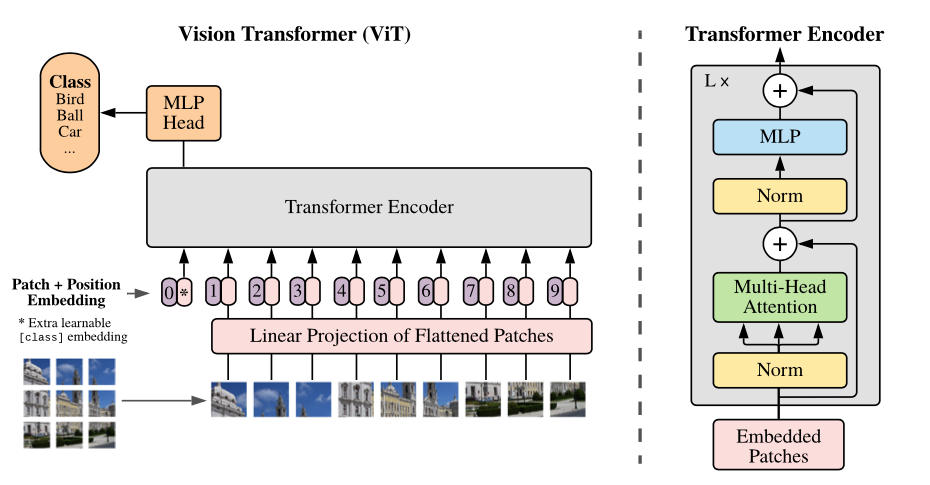
\includegraphics[width=0.95\textwidth]{vit_overview.png}
\caption{Kiến trúc Vision Transformer và một khối encoder. Nguồn: hình gốc trong repo \texttt{google-research/vision\_transformer} \cite{vitrepo}.}\label{fig:vit}
\end{figure}

\subsection{Mô hình thị giác--ngôn ngữ và CLIP}
CLIP dùng hai bộ mã hóa $f_I$ và $f_T$ cho ảnh và văn bản. Sau chuẩn hóa $L_2$, các vector của cặp phù hợp được đưa gần nhau trong không gian biểu diễn. Với một batch gồm $B$ cặp và hệ số $\alpha>0$, một chiều của hàm mất mát tương phản là \cite{clip}
\begin{equation}
\begin{gathered}
\mathcal L_{I\rightarrow T}=-\frac1B\sum_{i=1}^B
\log\frac{\exp(\alpha\,u_i^\top v_i)}{\sum_{j=1}^B\exp(\alpha\,u_i^\top v_j)},\\
u_i=\frac{f_I(I_i)}{\|f_I(I_i)\|_2},\quad v_i=\frac{f_T(t_i)}{\|f_T(t_i)\|_2}.
\end{gathered}
\end{equation}
CLIP kết hợp hai chiều ảnh--văn bản và văn bản--ảnh khi tiền huấn luyện. Khi phân loại zero-shot, mỗi tên lớp được đặt trong prompt, mã hóa thành vector và so sánh với ảnh. Hình~\ref{fig:clip} phân biệt tiền huấn luyện với suy luận. Đề tài chỉ sử dụng checkpoint đã huấn luyện, không chạy lại quá trình ở nửa trái của hình.
\begin{figure}[H]\centering
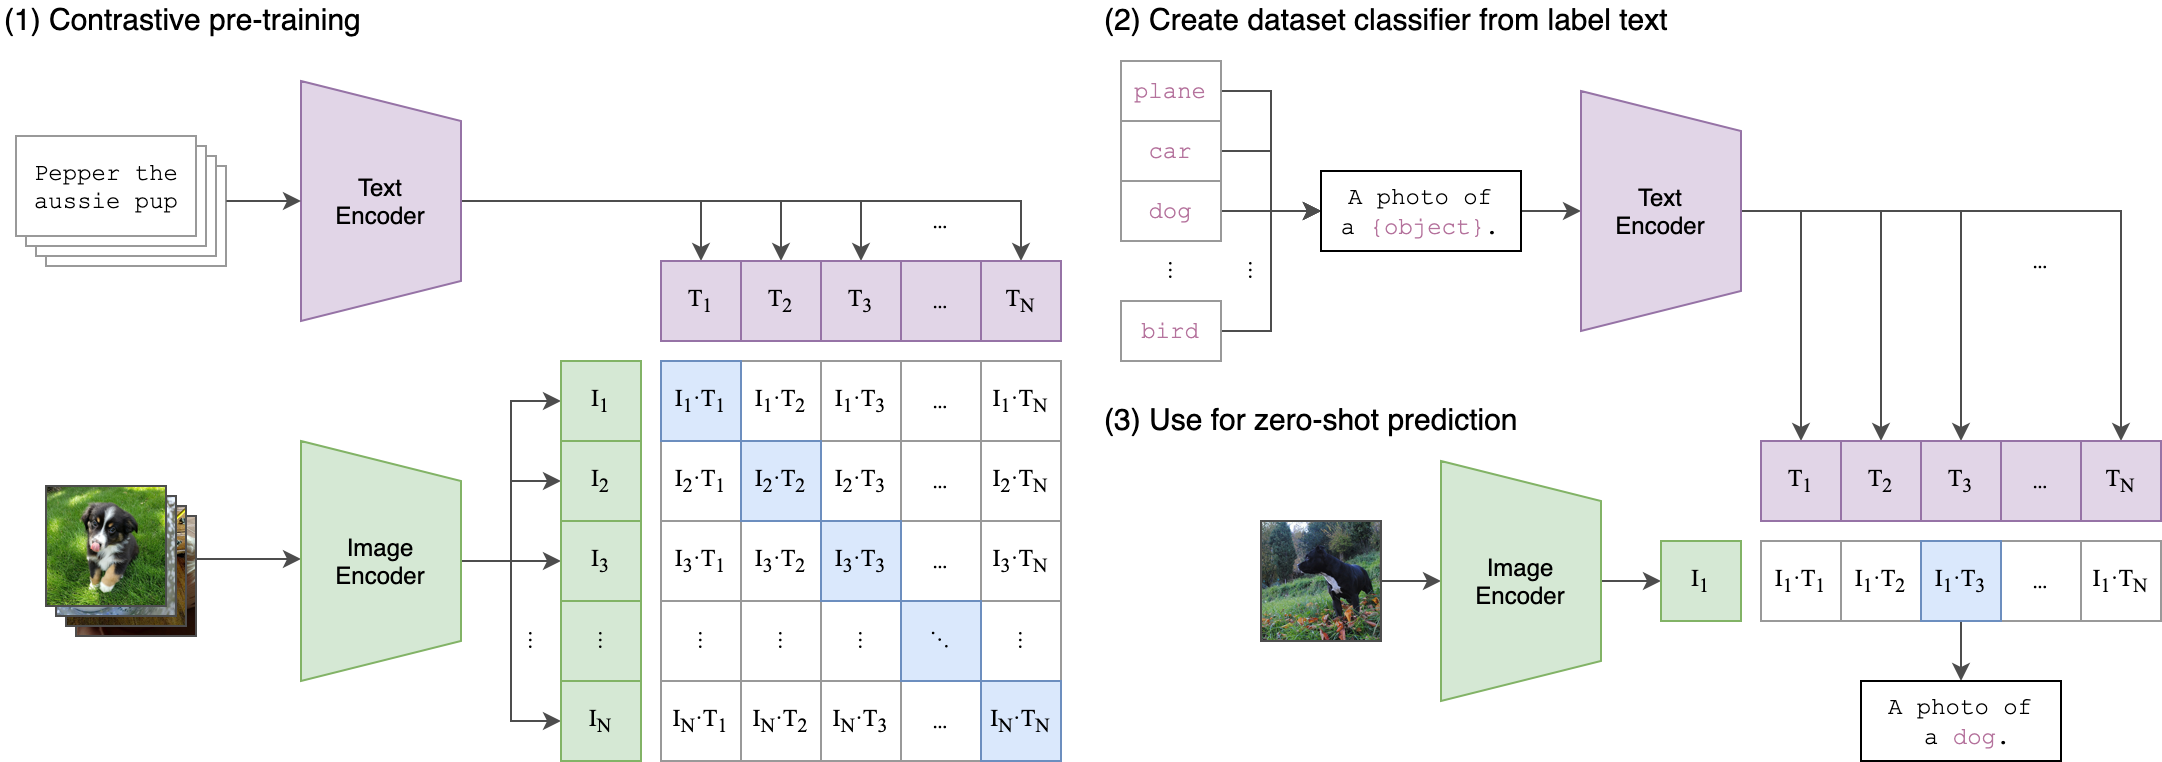
\includegraphics[width=\textwidth]{clip_overview.png}
\caption{Tiền huấn luyện tương phản và phân loại zero-shot bằng CLIP. Nguồn: hình \texttt{CLIP.png} trong repo OpenAI CLIP \cite{cliprepo}.}\label{fig:clip}
\end{figure}

\subsection{Các backbone được sử dụng}
Bốn backbone có chung giao diện mã hóa nhưng khác dữ liệu, tokenizer và quy trình tiền huấn luyện. Bảng~\ref{tab:backbone} ghi đúng kiến trúc và checkpoint của mã dự án. Các thay đổi tiền huấn luyện không được triển khai lại trong thí nghiệm.
\begin{table}[H]\centering\small
\caption{Backbone và checkpoint dùng trong 28 lượt.}\label{tab:backbone}
\begin{tabular}{p{0.17\textwidth}p{0.43\textwidth}p{0.28\textwidth}}\toprule
\textbf{Backbone}&\textbf{Kiến trúc / checkpoint}&\textbf{Đặc điểm kế thừa}\\\midrule
MetaCLIP2&\path{ViT-H-14-worldwide-quickgelu}; \path{metaclip2_worldwide}&Quy trình tiền huấn luyện trên dữ liệu web nhiều ngôn ngữ \cite{metaclip2}.\\
DFN5B&\path{apple/DFN5B-CLIP-ViT-H-14}&CLIP ViT-H/14 học từ dữ liệu được lọc bằng DFN \cite{dfn}.\\
SigLIP2&\path{ViT-SO400M-14-SigLIP2}; \path{webli}&Mục tiêu sigmoid, kết hợp captioning, self-distillation và masked prediction trong tiền huấn luyện \cite{siglip2}.\\
OpenAI CLIP&\path{ViT-B-32}; \path{openai}&Backbone CLIP ViT-B/32 làm đối chiếu \cite{clip}.\\\bottomrule
\end{tabular}\end{table}
Tokenizer được dùng theo checkpoint: cửa sổ ghi nhận là 77 token cho MetaCLIP2, DFN5B, OpenAI CLIP và 64 token cho SigLIP2. Bộ tiền xử lý ảnh lấy từ backbone. Vì ảnh và văn bản có thể khác độ dài đầu vào, cùng batch size không có nghĩa cùng chi phí suy luận.

\subsection{Prompt và DCLIP}
Với lớp $c$, đặt $\mathcal P_c=\{q_{c,1},\ldots,q_{c,M_c}\}$ là tập prompt và $e(q)=f_T(q)/\|f_T(q)\|_2$. Dự án dùng hai cách tổng hợp:
\begin{align}
\bar q_c&=\frac1{M_c}\sum_{j=1}^{M_c}e(q_{c,j}) &&\text{(mean\_sim)},\\
\widetilde q_c&=\frac{\bar q_c}{\|\bar q_c\|_2} &&\text{(mean\_embed)}.
\end{align}
Với vector mẫu chuẩn hóa $u$, $u^\top\bar q_c$ bằng trung bình cosine với từng prompt. Chuẩn hóa lại vector trung bình ở mean\_embed có thể đổi thứ hạng lớp; hai phép gộp không được xem là tương đương.

DCLIP xây dựng descriptor nêu đặc trưng của từng lớp, sau đó tổng hợp mức phù hợp giữa ảnh và các descriptor \cite{dclip}. Hình~\ref{fig:dclip} cho thấy khác biệt giữa chỉ dùng tên lớp và dùng nhiều đặc trưng. Bài gốc dùng LLM để tạo mô tả; bộ descriptor của dự án được tạo trước theo định nghĩa taxonomy và lưu cố định, không phải danh sách GPT-3 của bài gốc.
\begin{figure}[H]\centering
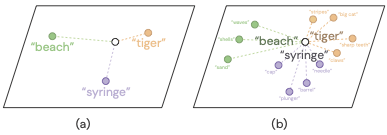
\includegraphics[width=0.72\textwidth]{dclip_descriptors.png}
\caption{(a) Đối chiếu với tên lớp; (b) đối chiếu với các descriptor. Nguồn: hình \texttt{figs/latent-points.png} trong repo Menon và Vondrick \cite{dcliprepo}.}\label{fig:dclip}
\end{figure}
Biến thể DCLIP adapted chỉ thay prompt nhánh ảnh và dùng mean\_sim cho nhánh này. Nhánh tweet vẫn sử dụng prompt baseline. Vì baseline CrisisMMD dùng mean\_embed, đối chứng hiện tại đo toàn bộ biến thể gồm \emph{nội dung descriptor và phép gộp}, chưa cô lập tác động riêng của nội dung mô tả.

\subsection{Độ đo đánh giá}
Với lớp $c$, Precision $P_c$, Recall $R_c$ và F1 được tính từ TP, FP, FN:
\begin{equation}
P_c=\frac{TP_c}{TP_c+FP_c},\quad R_c=\frac{TP_c}{TP_c+FN_c},\quad
F1_c=\frac{2TP_c}{2TP_c+FP_c+FN_c}.
\end{equation}
Khi mẫu số bằng 0, kết quả được quy ước bằng 0. Với $C=|\mathcal C|$ lớp,
\begin{equation}
\operatorname{MacroF1}=\frac1C\sum_cF1_c,\quad
\operatorname{BA}=\frac1C\sum_cR_c,\quad
\operatorname{Accuracy}=\frac1N\sum_i\mathbf1[\hat y_i=y_i].
\end{equation}
Macro-F1 cho mỗi lớp trọng số bằng nhau nhưng vẫn nhạy với lớp có ít quan sát. BA bổ sung góc nhìn Recall; Accuracy phản ánh số bản ghi đúng và có thể bị chi phối bởi lớp lớn.

Đối với MM-IMDb, Micro-F1 gộp TP, FP, FN qua tất cả cặp mẫu--nhãn; Samples-F1 lấy trung bình F1 của tập nhãn trên từng phim:
\begin{equation}
\operatorname{SamplesF1}=\frac1N\sum_i\frac{2|Y_i\cap\hat Y_i|}{|Y_i|+|\hat Y_i|}.
\end{equation}
Hamming Accuracy là tỷ lệ quyết định có/không thuộc lớp được dự đoán đúng; Exact Match yêu cầu cả tập nhãn đúng hoàn toàn. Không dùng Hamming Accuracy đơn lẻ để kết luận vì đa số cặp mẫu--nhãn là âm tính.

\newpage
\section{Chương 3: MÔ HÌNH ĐỀ XUẤT}
\subsection{Kiến trúc hệ thống}
Hệ thống nhận một cặp ảnh--văn bản cùng bộ prompt cố định. Mỗi nhánh tạo vector mẫu và tính điểm với biểu diễn lớp. Hình~\ref{fig:system} mô tả đúng luồng suy luận đã triển khai. Hai ô text encoder dùng chung trọng số $f_T$ nhưng nhận văn bản mẫu và prompt lớp tương ứng. Bộ mã hóa giữ nguyên trọng số; nhãn thật chỉ đi vào khối đánh giá \cite{internal}.
\begin{figure}[H]\centering
\begin{tikzpicture}[font=\linespread{1}\fontsize{10}{12}\selectfont,>=Latex,
 box/.style={draw,rounded corners=2pt,align=center,text width=3.0cm,minimum height=0.95cm,fill=blue!5},
 processbox/.style={box,fill=green!6}, target/.style={box,dashed,fill=orange!8}]
\node[box] (im) at (0,0) {Ảnh $I$};
\node[box] (tx) at (4.4,0) {Văn bản $t$};
\node[box] (pr) at (8.8,0) {Nhãn lớp\\và prompt cố định};
\node[processbox] (ie) at (0,-1.6) {Image encoder $f_I$\\chuẩn hóa $L_2$};
\node[processbox] (te) at (4.4,-1.6) {Text encoder $f_T$\\chunking nếu cần};
\node[processbox,text width=3.3cm] (qe) at (8.8,-1.6) {Text encoder $f_T$\\tạo $q_c^I,q_c^T$};
\node[box] (si) at (0,-3.5) {$s_I(c)=u^\top q_c^I$};
\node[box] (st) at (4.4,-3.5) {$s_T(c)=v^\top q_c^T$};
\node[box] (pi) at (0,-5) {Softmax\\hoặc relative-z};
\node[box] (pt) at (4.4,-5) {Softmax\\hoặc relative-z};
\node[processbox,text width=4.8cm] (fu) at (2.2,-6.6) {Fusion cố định\\$w\,a_I(c)+(1-w)\,a_T(c)$};
\node[box,text width=4.8cm] (de) at (2.2,-8.2) {Một nhãn: argmax\\Nhiều nhãn: ngưỡng và top-1 dự phòng};
\node[target] (gt) at (8.8,-5.4) {Nhãn thật $y$ / $Y$\\chỉ dùng đánh giá};
\node[box,fill=orange!8] (ev) at (8.8,-8.2) {Đánh giá\\và lưu kết quả};
\draw[->] (im)--(ie); \draw[->] (tx)--(te); \draw[->] (pr)--(qe);
\draw[->] (ie)--(si); \draw[->] (te)--(st);
\draw[->] (qe.south)--(8.8,-2.5)-|(si.north);
\draw[->] (qe.south)--(8.8,-2.9)-|(st.north);
\draw[->] (si)--(pi); \draw[->] (st)--(pt);
\draw[->] (pi.south)--(0,-5.8)-|(fu.north);
\draw[->] (pt.south)--(4.4,-6.0)-|(fu.north);
\draw[->] (fu)--(de); \draw[->] (de)--(ev); \draw[->,dashed] (gt)--(ev);
\end{tikzpicture}
\caption{Kiến trúc hệ thống do nhóm vẽ bằng TikZ theo mã triển khai. DCLIP thay $q_c^I$; $q_c^T$ giữ prompt baseline. Nhãn thật không tham gia tạo điểm.}\label{fig:system}
\end{figure}

\subsection{Suy luận cho bài toán một nhãn}
Với Fakeddit và CrisisMMD, mỗi nhánh được chuyển thành phân phối điểm trên các lớp:
\begin{equation}
p_I(c)=\operatorname{softmax}_c(\alpha_I s_I(c)+b_I),\quad
p_T(c)=\operatorname{softmax}_c(\alpha_T s_T(c)+b_T).
\end{equation}
Hệ số nhánh ảnh lấy từ checkpoint. Nhánh văn bản Fakeddit dùng scale 25; CrisisMMD dùng scale của checkpoint. Cả bốn backbone đều dùng softmax trong các task một nhãn, kể cả SigLIP2; đây là quy tắc suy luận của dự án, khác với mục tiêu sigmoid khi tiền huấn luyện SigLIP2.
\begin{equation}
p(c)=w\,p_I(c)+(1-w)\,p_T(c),\qquad \hat y=\arg\max_c p(c).
\end{equation}
Trọng số $w=0,75$ cho Fakeddit và $w=0,5$ cho CrisisMMD. Không học trọng số bằng nhãn đánh giá. Nếu văn bản rỗng, hệ thống dùng nhánh ảnh; kiểm tra 28 lượt không ghi nhận mẫu văn bản rỗng. Điểm softmax được dùng để kết hợp và xếp hạng, không mặc định là xác suất đã hiệu chuẩn.

\subsection{Suy luận nhiều nhãn và văn bản dài}
MM-IMDb dùng relative-z: chuẩn hóa điểm cosine theo 23 lớp \emph{trong từng mẫu và từng nhánh}, không dùng trung bình hoặc phương sai của toàn bộ dataset:
\begin{equation}
z_m(c)=\frac{s_m(c)-\mu_m}{\sigma_m},\quad m\in\{I,T\};\qquad
z(c)=0,5z_I(c)+0,5z_T(c).
\end{equation}
Nếu phương sai bằng 0, nhánh được gán vector 0. Chọn các lớp có $z(c)>1,0$; nếu không có lớp nào vượt ngưỡng thì chọn lớp điểm cao nhất. Điểm z không phải xác suất. Với quy tắc này, scale, bias và ngưỡng sigmoid 0,22 không tham gia quyết định nhãn.

Plot vượt cửa sổ tokenizer được chia theo câu; câu quá dài tiếp tục chia theo từ hoặc ký tự. Mỗi đoạn được mã hóa trong cửa sổ cho phép. Các embedding đoạn được lấy trung bình và chuẩn hóa lại $L_2$. Tham số \path{chunk_aggregation=mean_embed} được giữ trong cả bốn lượt MM-IMDb. Đây là gộp các đoạn của văn bản mẫu, khác với gộp nhiều prompt của một lớp.

\subsection{Quy trình triển khai và lưu vết}
Trước khi nạp mô hình, worker Kaggle kiểm tra hash gói mã/dữ liệu, cohort ID, ID bản ghi, nhãn và số mẫu. Sau suy luận, hệ thống lưu summary, dự đoán từng mẫu, điểm từng nhánh, snapshot cấu hình và receipt GPU. Các cấu hình so sánh trong một task được đối chiếu theo nội dung mẫu, không chỉ theo tên thư mục hoặc fingerprint chứa thời gian tệp.

\begin{algorithm}[H]
\caption{Quy trình đánh giá một cấu hình zero-shot}
\KwIn{Bộ mẫu có nhãn thật; checkpoint; prompt; trọng số và quy tắc quyết định cố định}
\KwOut{Chỉ số, dự đoán, điểm nhánh và biên nhận thực thi}
Xác thực bộ mẫu và khóa danh sách ID\;
Nạp checkpoint, giữ nguyên trọng số; mã hóa prompt lớp\;
Mã hóa ảnh và văn bản; chia plot dài nếu được cấu hình\;
Tính điểm từng nhánh, kết hợp và quyết định nhãn\;
Đối chiếu dự đoán với nhãn thật; tính chỉ số\;
Lưu cấu hình hiệu lực, log và receipt\;
\end{algorithm}

\newpage
\section{Chương 4: THỰC NGHIỆM}
\subsection{Dữ liệu thực nghiệm}
Chỉ ba cohort chính, mỗi cohort 3.000 bản ghi, được sử dụng trong phần kết quả. Fakeddit và CrisisMMD mỗi bộ dùng chung mẫu giữa hai task; do đó có 9.000 bản ghi thuộc ba nguồn và 15.000 cặp bản ghi--task, không phải 15.000 ảnh riêng biệt. Đặc tả nguồn và kiểm tra ảnh được lưu cùng dự án \cite{dataaudit}.
\begin{table}[H]\centering\small
\caption{Nguồn dữ liệu và đơn vị đánh giá.}\label{tab:data}
\begin{tabular}{p{0.16\textwidth}p{0.18\textwidth}p{0.51\textwidth}}\toprule
\textbf{Dataset}&\textbf{Nguồn / N}&\textbf{Task và cách chọn mẫu}\\\midrule
Fakeddit&Validation / 3.000&Tiêu đề Reddit--ảnh; quota theo sáu lớp trong pool hợp lệ, dùng cho 2way/6way.\\
CrisisMMD&Train chung / 3.000&Tweet--ảnh; chọn từ 10.433 cặp thuộc train chung hai task; phân tầng nhãn và sự kiện, seed 42.\\
MM-IMDb&Test / 3.000&Plot--poster; chọn trong 7.799 phim test đủ cặp; phân tầng lặp theo nhiều nhãn, seed 42 \cite{multilabel-stratification}.\\
\bottomrule\end{tabular}\end{table}

\subsubsection{Fakeddit}
Fakeddit là dữ liệu Reddit với nhãn được xây dựng bằng distant supervision \cite{fakeddit}. Dự án dùng \path{clean_title}, giữ tiêu đề có \path{len(text.replace(" ", "")) > 20}, tức ít nhất 21 ký tự không tính dấu cách. Bộ mẫu có đủ 3.000 ảnh đã kiểm tra giải mã; ảnh thông báo liên kết đã bị xóa được loại trong bước chuẩn bị. Hai task dùng cùng 3.000 bản ghi. Nhãn 2way là Fake (giả): 1.463 và Real (thật): 1.537. ID 0 của 2way là Fake, trong khi ID 0 của 6way là True.
\begin{table}[H]\centering\small
\caption{Nhãn và phân bố Fakeddit 6way.}\label{tab:fakeddit-support}
\begin{tabular}{cp{0.70\textwidth}r}\toprule
\textbf{ID}&\textbf{Nhãn}&\textbf{Support}\\\midrule
0&\ClassLabel{True}{Thật}&1.537\\
1&\ClassLabel{Satire/Parody}{Châm biếm/nhại}&204\\
2&\ClassLabel{False Connection}{Liên kết sai}&602\\
3&\ClassLabel{Imposter Content}{Nội dung mạo danh}&92\\
4&\ClassLabel{Manipulated Content}{Nội dung bị chỉnh sửa}&407\\
5&\ClassLabel{Misleading Content}{Nội dung gây hiểu lầm}&158\\
\bottomrule\end{tabular}\end{table}

\subsubsection{CrisisMMD}
CrisisMMD có annotation ảnh và văn bản riêng cho các nhiệm vụ hỗ trợ ứng phó thiên tai \cite{crisismmd}. Dự án dùng \emph{nhãn ảnh} làm đích đánh giá: \path{label_informative} hoặc \path{label_humanitarian}, với khóa bản ghi \path{image_id}. Hai nhãn được giữ trên cùng 3.000 cặp từ phần train chung; không cập nhật trọng số mô hình trên train này. Kết quả là khảo sát zero-shot trên train nguồn, không phải điểm test chính thức.

Informativeness gồm 1.551 Informative (có thông tin hữu ích) và 1.449 Not Informative (không có thông tin hữu ích). Bộ mẫu bao phủ bảy sự kiện: California Wildfires 243, Hurricane Harvey 721, Hurricane Irma 753, Hurricane Maria 769, Iraq--Iran Earthquake 101, Mexico Earthquake 229 và Sri Lanka Floods 184. Phân bố humanitarian được nêu tại Bảng~\ref{tab:human-support}.
\begin{table}[H]\centering\small
\caption{Phân bố nhãn humanitarian trên cùng bộ mẫu CrisisMMD.}\label{tab:human-support}
\begin{tabular}{p{0.76\textwidth}r}\toprule
\textbf{Nhãn}&\textbf{Support}\\\midrule
\ClassLabel{Not Humanitarian}{Không thuộc nhóm thông tin nhân đạo}&1.449\\
\ClassLabel{Other Relevant Information}{Thông tin liên quan khác}&404\\
\ClassLabel{Rescue, Volunteering or Donation Effort}{Cứu hộ, tình nguyện hoặc quyên góp}&382\\
\ClassLabel{Infrastructure and Utility Damage}{Thiệt hại hạ tầng và tiện ích}&603\\
\ClassLabel{Affected Individuals}{Người bị ảnh hưởng}&86\\
\ClassLabel{Vehicle Damage}{Thiệt hại phương tiện}&52\\
\ClassLabel{Injured or Dead People}{Người bị thương hoặc tử vong}&22\\
\ClassLabel{Missing or Found People}{Người mất tích hoặc được tìm thấy}&2\\
\bottomrule\end{tabular}\end{table}

\subsubsection{MM-IMDb và tính đại diện của mẫu}
MM-IMDb ghép poster và plot với nhiều nhãn thể loại \cite{mmimdb}. Bộ mẫu giữ 23 genre, trung bình 2,484 nhãn/phim. Drama (chính kịch) có 1.595 mẫu và Comedy (hài) có 1.004; Film-Noir (phim noir) chỉ có 39, Short (phim ngắn) 55. Support đầy đủ được trình bày cùng phân tích từng genre ở Bảng~\ref{tab:mm-perclass}.

Ba bộ mẫu giữ gần phân bố nguồn hợp lệ thay vì cân bằng đều các lớp. Điều kiện có ảnh đọc được và văn bản hợp lệ có thể tạo thiên lệch so với toàn bộ dữ liệu nguồn. Có 3.000 ID riêng biệt ở mỗi bộ, nhưng số checksum ảnh khác nhau lần lượt là 2.998, 2.983 và 2.998 cho Fakeddit, CrisisMMD và MM-IMDb; không đồng nhất số bản ghi với số nội dung ảnh độc lập \cite{dataaudit}.

\subsection{Cài đặt và kiểm tra thực nghiệm}
\subsubsection{Ma trận và cấu hình hiệu lực}
Năm task nhân bốn backbone tạo 20 lượt baseline. Hai task CrisisMMD nhân bốn backbone tạo thêm tám lượt DCLIP adapted. Tất cả receipt ghi GPU thực tế là \textbf{Tesla T4}; batch size là 16. Mã nguồn dùng Python, PyTorch, OpenCLIP và scikit-learn. Các lượt có cùng checksum gói mã; không suy diễn cùng checksum mã thành môi trường thư viện được ghim hoàn toàn.
\begin{table}[H]\centering\small
\caption{Cấu hình quyết định nhãn của các lượt đã chạy.}\label{tab:settings}
\begin{tabular}{p{0.19\textwidth}p{0.32\textwidth}p{0.35\textwidth}}\toprule
\textbf{Nhóm}&\textbf{Prompt / fusion}&\textbf{Quyết định nhãn}\\\midrule
Fakeddit baseline&mean\_sim; $w_I=0,75$, scale text 25.&Softmax từng nhánh; argmax sau fusion.\\
CrisisMMD baseline&mean\_embed; $w_I=0,5$, scale theo checkpoint.&Softmax từng nhánh; argmax sau fusion.\\
CrisisMMD DCLIP&Ảnh: descriptor + mean\_sim. Text và fusion giữ baseline.&Cùng tập nhãn, bộ mẫu và quy tắc argmax.\\
MM-IMDb baseline&mean\_sim; $w_I=0,5$; plot dài chia đoạn rồi mean\_embed.&Relative-z, ngưỡng $>1,0$; top-1 dự phòng.\\
\bottomrule\end{tabular}\end{table}

Các lượt đều tắt heuristic quan hệ ảnh--văn bản và ensemble giữa backbone. Không thực hiện tìm ngưỡng hoặc huấn luyện thêm trong quy trình đánh giá. Descriptor của hai task CrisisMMD được giữ cố định trong từng nhóm đối chứng.

\subsubsection{Xác thực số liệu trước khi phân tích}
Tập kết quả được kiểm tra bằng \path{scripts/analyze_report_3000.py}. Mỗi lượt phải có receipt đúng cohort, đủ 3.000 ID riêng biệt, điểm hữu hạn và dự đoán khớp quy tắc quyết định. Tính lại Accuracy/F1 từ 84.000 dòng dự đoán cho kết quả khớp summary trong sai số $10^{-10}$ đối với các chỉ số được lưu. BA, Hamming Accuracy, Exact Match và F1 từng lớp được tính từ cùng các dự đoán, không chạy lại mô hình \cite{resultaudit}.

Trong cùng task, các lượt có cùng ID, nhãn, hash văn bản, tên/kích thước ảnh và checksum gói dữ liệu. Tám cặp baseline--DCLIP có điểm nhánh tweet trùng từng mẫu; chỉ nhánh ảnh được thay đổi. Snapshot vẫn ghi \path{split_verified=false} vì runner không tự xác minh nguồn split; tên split của báo cáo dựa trên hồ sơ chuẩn bị dữ liệu và receipt, không dựa vào cờ này.

Các bảng kết quả bên dưới dùng đơn vị \textbf{\%}; chênh lệch giữa hai tỷ lệ được diễn đạt bằng \textbf{điểm phần trăm}. Nhánh ảnh và nhánh text được đánh giá lại từ điểm đã lưu trong cùng lượt, không phải thí nghiệm huấn luyện riêng.

\subsection{Kết quả Fakeddit}
\begin{table}[H]\centering\small
\caption{Kết quả baseline Fakeddit trên 3.000 mẫu dùng chung hai task (\%).}\label{tab:fk-results}
\begin{tabular}{lrrrrrr}\toprule
&\multicolumn{3}{c}{\textbf{2way}}&\multicolumn{3}{c}{\textbf{6way}}\\\cmidrule(lr){2-4}\cmidrule(lr){5-7}\textbf{Backbone}&\textbf{Acc.}&\textbf{Macro-F1}&\textbf{BA}&\textbf{Acc.}&\textbf{Macro-F1}&\textbf{BA}\\\midrule
MetaCLIP2&54,20&50,36&53,55&34,87&25,20&29,39\\
DFN5B&53,10&45,07&52,19&28,70&21,35&22,95\\
SigLIP2&52,23&42,18&51,24&41,13&25,58&26,12\\
OpenAI CLIP&42,17&34,04&43,06&23,00&20,60&28,60\\
\bottomrule\end{tabular}\end{table}

MetaCLIP2 có Macro-F1 cao nhất ở 2way, đạt 50,36\%. Ở 6way, SigLIP2 đứng đầu Macro-F1 với 25,58\%, rất gần MetaCLIP2 25,20\%; MetaCLIP2 có BA cao hơn, 29,39\% so với 26,12\%. Vì vậy, thứ hạng còn phụ thuộc chỉ số.

Một quy tắc luôn đoán lớp lớn nhất đạt Accuracy 51,23\% ở cả hai task. Các backbone 2way chỉ cao hơn nhẹ hoặc thấp hơn mốc này; ở 6way, toàn bộ Accuracy thấp hơn mốc lớp lớn nhất. Tuy nhiên, Macro-F1 mốc 6way chỉ là 11,29\%, thấp hơn các mô hình, vì quy tắc đó bỏ qua năm lớp còn lại. Kết quả cho thấy mô hình có phân biệt nhiều lớp nhưng chưa giải quyết tốt bài toán thật--giả và các loại sai lệch.
\begin{table}[H]\centering\small
\caption{F1 từng lớp Fakeddit 6way của SigLIP2 (\%).}\label{tab:fk-perclass}
\begin{tabular}{p{0.47\textwidth}rrrr}\toprule
\textbf{Lớp}&\textbf{Support}&\textbf{Precision}&\textbf{Recall}&\textbf{F1}\\\midrule
\ClassLabel{True}{Thật}&1.537&57,63&49,64&53,34\\
\ClassLabel{Satire/Parody}{Châm biếm/nhại}&204&8,27&5,39&6,53\\
\ClassLabel{False Connection}{Liên kết sai}&602&22,57&36,21&27,81\\
\ClassLabel{Imposter Content}{Nội dung mạo danh}&92&3,80&3,26&3,51\\
\ClassLabel{Manipulated Content}{Nội dung bị chỉnh sửa}&407&50,44&56,51&53,30\\
\ClassLabel{Misleading Content}{Nội dung gây hiểu lầm}&158&21,43&5,70&9,00\\
\bottomrule\end{tabular}\end{table}

SigLIP2 đạt F1 khoảng 53\% ở True và Manipulated Content, nhưng chỉ 3,51\% ở Imposter Content và 6,53\% ở Satire/Parody. Chênh lệch này giải thích Macro-F1 thấp dù lớp True có support lớn. Tương đồng ảnh với mô tả chưa cung cấp đầy đủ bằng chứng về nguồn tin, mạo danh hoặc dụng ý châm biếm. Đây là giới hạn được gợi ra bởi kết quả; chưa phải kết luận nguyên nhân cho từng mẫu lỗi.

\subsection{Kết quả CrisisMMD và đối chứng DCLIP}
\begin{table}[H]\centering\small
\caption{Informativeness: cùng 3.000 mẫu, cùng backbone giữa hai phương pháp (\%).}\label{tab:crisis-info}
\begin{tabular}{lrrrrrr}\toprule
&\multicolumn{3}{c}{\textbf{Baseline}}&\multicolumn{3}{c}{\textbf{DCLIP adapted}}\\\cmidrule(lr){2-4}\cmidrule(lr){5-7}\textbf{Backbone}&\textbf{Acc.}&\textbf{Macro-F1}&\textbf{BA}&\textbf{Acc.}&\textbf{Macro-F1}&\textbf{BA}\\\midrule
MetaCLIP2&73,10&72,07&72,53&74,03&72,63&73,35\\
DFN5B&71,37&70,74&71,95&71,67&71,40&72,08\\
SigLIP2&69,27&68,05&70,01&67,67&66,21&68,45\\
OpenAI CLIP&73,47&71,46&72,65&77,47&76,57&76,89\\
\bottomrule\end{tabular}\end{table}
\begin{table}[H]\centering\small
\caption{Humanitarian: cùng 3.000 mẫu, cùng backbone giữa hai phương pháp (\%).}\label{tab:crisis-human}
\begin{tabular}{lrrrrrr}\toprule
&\multicolumn{3}{c}{\textbf{Baseline}}&\multicolumn{3}{c}{\textbf{DCLIP adapted}}\\\cmidrule(lr){2-4}\cmidrule(lr){5-7}\textbf{Backbone}&\textbf{Acc.}&\textbf{Macro-F1}&\textbf{BA}&\textbf{Acc.}&\textbf{Macro-F1}&\textbf{BA}\\\midrule
MetaCLIP2&55,43&37,80&45,91&54,03&37,90&43,22\\
DFN5B&57,63&40,61&50,59&59,07&42,22&46,20\\
SigLIP2&57,53&33,85&34,67&59,00&37,62&36,91\\
OpenAI CLIP&53,07&37,09&48,61&58,43&40,86&45,42\\
\bottomrule\end{tabular}\end{table}

Trên informativeness, baseline MetaCLIP2 có Macro-F1 cao nhất là 72,07\%. Với DCLIP adapted, OpenAI CLIP đạt 76,57\%, tăng 5,11 điểm phần trăm so với baseline cùng backbone. MetaCLIP2 và DFN5B tăng lần lượt 0,56 và 0,66 điểm; SigLIP2 giảm 1,83 điểm.

Trên humanitarian, DFN5B có Macro-F1 tốt nhất trong cả baseline (40,61\%) và DCLIP adapted (42,22\%). OpenAI CLIP tăng từ 37,09\% lên 40,86\%; SigLIP2 tăng từ 33,85\% lên 37,62\%. MetaCLIP2 chỉ tăng khoảng 0,10 điểm Macro-F1 trong khi Accuracy giảm 1,40 điểm. Không có một backbone tốt nhất cho mọi task.

Đối chiếu từng mẫu cho thấy OpenAI CLIP+DCLIP informativeness sửa 223 dự đoán sai và tạo 103 lỗi mới, tăng ròng 120 mẫu đúng. SigLIP2 trên cùng task sửa 166 nhưng tạo 214 lỗi mới, giảm ròng 48. Với DFN5B humanitarian, số sửa/tạo lỗi là 226/183. Đây là số thay đổi dự đoán quan sát được, chưa là kiểm định ý nghĩa thống kê hoặc bằng chứng hiệu quả trên dữ liệu ngoài cohort.
\begin{table}[H]\centering\small
\caption{DFN5B humanitarian: F1 và Recall từng lớp trước/sau DCLIP (\%).}\label{tab:human-perclass}
\begin{tabular}{p{0.48\textwidth}rrrrr}\toprule
\textbf{Lớp}&\textbf{N}&\textbf{F1 B}&\textbf{F1 D}&\textbf{R B}&\textbf{R D}\\\midrule
\ClassLabel{Not Humanitarian}{Không thuộc nhóm thông tin nhân đạo}&1.449&67,53&66,45&66,60&64,80\\
\ClassLabel{Other Relevant Information}{Thông tin liên quan khác}&404&64,12&68,99&53,96&66,09\\
\ClassLabel{Rescue, Volunteering or Donation Effort}{Cứu hộ, tình nguyện hoặc quyên góp}&382&53,73&51,03&67,02&64,66\\
\ClassLabel{Infrastructure and Utility Damage}{Thiệt hại hạ tầng và tiện ích}&603&46,15&54,08&33,83&42,29\\
\ClassLabel{Affected Individuals}{Người bị ảnh hưởng}&86&30,30&29,85&40,70&34,88\\
\ClassLabel{Vehicle Damage}{Thiệt hại phương tiện}&52&38,42&36,97&65,38&42,31\\
\ClassLabel{Injured or Dead People}{Người bị thương hoặc tử vong}&22&24,64&30,38&77,27&54,55\\
\ClassLabel{Missing or Found People}{Người mất tích hoặc được tìm thấy}&2&0,00&0,00&0,00&0,00\\
\bottomrule\end{tabular}\end{table}

Trong Bảng~\ref{tab:human-perclass}, B là baseline, D là DCLIP adapted, R là Recall. DCLIP cải thiện F1 hạ tầng từ 46,15\% lên 54,08\% và thông tin liên quan khác từ 64,12\% lên 68,99\%. Tuy nhiên, Recall lớp Vehicle Damage giảm từ 65,38\% xuống 42,31\%, và Injured or Dead People giảm từ 77,27\% xuống 54,55\%. Vì vậy BA giảm từ 50,59\% xuống 46,20\% dù Macro-F1 tăng. Lớp Missing or Found People có hai mẫu và F1 bằng 0 ở cả hai cấu hình; chưa thể kết luận khả năng nhận diện lớp này ở mức quần thể.

\subsection{Kết quả MM-IMDb}
\begin{table}[H]\centering\small
\caption{MM-IMDb: kết quả nhiều nhãn trên 3.000 phim test (\%).}\label{tab:mm-results}
\begin{tabular}{lrrrrr}\toprule
\textbf{Backbone}&\textbf{Micro-F1}&\textbf{Macro-F1}&\textbf{Samples-F1}&\textbf{Hamming Acc.}&\textbf{Exact}\\\midrule
MetaCLIP2&51,23&51,18&50,18&88,13&3,20\\
DFN5B&44,58&43,04&42,65&86,71&1,97\\
SigLIP2&46,08&48,64&44,08&87,44&3,10\\
OpenAI CLIP&42,12&38,03&40,61&86,87&2,40\\
\bottomrule\end{tabular}\end{table}

MetaCLIP2 đạt cao nhất theo Micro-F1 51,23\%, Macro-F1 51,18\% và Samples-F1 50,18\%. SigLIP2 xếp thứ hai về Macro-F1, đạt 48,64\%. Exact Match chỉ từ 1,97\% đến 3,20\%, cho thấy dự đoán đúng toàn bộ tập thể loại của một phim vẫn khó.

Hamming Accuracy nằm trong khoảng 86,71--88,13\%, nhưng quy tắc không gán nhãn nào đã đạt 89,20\% vì mỗi phim chỉ có trung bình 2,484 nhãn trên 23 lớp. Quy tắc đó có F1 bằng 0. Do vậy, điểm Hamming cao không thay thế được Micro-/Macro-F1. Các mô hình dự đoán trung bình 2,735--3,112 nhãn/phim, cao hơn nhãn thật; có hiện tượng gán thừa nhãn.
\begin{table}[H]\centering\small
\caption{Support và kết quả từng genre của MetaCLIP2 trên MM-IMDb (\%).}\label{tab:mm-perclass}
\begin{tabular}{p{0.46\textwidth}rrrr}\toprule
\textbf{Genre (thể loại)}&\textbf{Support}&\textbf{Precision}&\textbf{Recall}&\textbf{F1}\\\midrule
Action (Hành động)&402&72,64&59,45&65,39\\
Adventure (Phiêu lưu)&316&72,73&10,13&17,78\\
Animation (Hoạt hình)&118&91,30&35,59&51,22\\
Biography (Tiểu sử)&158&17,52&68,99&27,95\\
Comedy (Hài)&1.004&91,12&46,02&61,15\\
Crime (Tội phạm)&447&62,62&59,96&61,26\\
Documentary (Tài liệu)&242&88,20&58,68&70,47\\
Drama (Chính kịch)&1.595&71,53&65,52&68,39\\
Family (Gia đình)&199&52,73&72,86&61,18\\
Fantasy (Kỳ ảo)&225&49,24&43,11&45,97\\
Film-Noir (Phim noir)&39&2,39&100,00&4,67\\
History (Lịch sử)&133&36,57&48,12&41,56\\
Horror (Kinh dị)&317&76,97&80,13&78,52\\
Music (Âm nhạc)&120&75,00&47,50&58,16\\
Musical (Nhạc kịch)&97&32,59&45,36&37,93\\
Mystery (Bí ẩn)&237&30,75&53,59&39,08\\
Short (Phim ngắn)&55&4,83&45,45&8,73\\
Romance (Lãng mạn)&612&46,61&65,20&54,36\\
Sci-Fi (Khoa học viễn tưởng)&225&82,93&45,33&58,62\\
Sport (Thể thao)&73&55,88&78,08&65,14\\
Thriller (Giật gân)&603&60,32&63,02&61,64\\
War (Chiến tranh)&154&57,71&65,58&61,40\\
Western (Cao bồi)&81&68,63&86,42&76,50\\
\bottomrule\end{tabular}\end{table}

MetaCLIP2 đạt F1 cao ở Horror (78,52\%) và Western (76,50\%), nhưng thấp ở Film-Noir (4,67\%), Short (8,73\%) và Adventure (17,78\%). Film-Noir có Recall 100\% nhưng Precision chỉ 2,39\%: mô hình tìm đủ 39 mẫu dương nhưng gán nhãn này quá rộng. Ngưỡng relative-z cố định vì vậy chưa phù hợp đồng đều cho mọi genre.

Khoảng 1.823--1.915 plot vượt cửa sổ tokenizer tùy backbone và đã được chia đoạn. Các số \path{n_truncated} trong audit đo độ dài \emph{văn bản gốc}; với chunking bật, không được diễn giải chúng là số plot bị mất toàn bộ phần đuôi. Tổng số đoạn lần lượt là 6.167 (MetaCLIP2), 6.127 (DFN5B/OpenAI CLIP) và 6.408 (SigLIP2).

\subsection{Đóng góp của nhánh ảnh, văn bản và fusion}
\begin{table}[H]\centering\small
\caption{Macro-F1 từng nhánh và fusion của 20 lượt baseline (\%).}\label{tab:branches}
\begin{tabular}{llrrr}\toprule
\textbf{Task}&\textbf{Backbone}&\textbf{Ảnh}&\textbf{Text}&\textbf{Fusion}\\\midrule
Fakeddit 2way&MetaCLIP2&52,93&38,51&50,36\\
&DFN5B&48,61&42,67&45,07\\
&SigLIP2&44,65&37,60&42,18\\
&OpenAI CLIP&34,08&36,91&34,04\\
\midrule
Fakeddit 6way&MetaCLIP2&25,61&10,26&25,20\\
&DFN5B&19,80&12,20&21,35\\
&SigLIP2&26,04&13,57&25,58\\
&OpenAI CLIP&20,40&11,27&20,60\\
\midrule
Informativeness&MetaCLIP2&78,19&61,13&72,07\\
&DFN5B&72,71&63,93&70,74\\
&SigLIP2&74,78&58,48&68,05\\
&OpenAI CLIP&71,89&64,84&71,46\\
\midrule
Humanitarian&MetaCLIP2&42,40&25,85&37,80\\
&DFN5B&41,12&26,49&40,61\\
&SigLIP2&43,14&19,86&33,85\\
&OpenAI CLIP&31,43&24,82&37,09\\
\midrule
MM-IMDb&MetaCLIP2&44,78&42,62&51,18\\
&DFN5B&37,81&37,76&43,04\\
&SigLIP2&40,56&40,28&48,64\\
&OpenAI CLIP&35,18&33,44&38,03\\
\bottomrule\end{tabular}\end{table}

Fusion vượt cả hai nhánh trong bảy trên 20 cấu hình baseline: cả bốn backbone MM-IMDb, DFN5B/OpenAI CLIP Fakeddit 6way và OpenAI CLIP humanitarian. Ngược lại, ở Fakeddit 2way và CrisisMMD informativeness, fusion thấp hơn nhánh ảnh ở cả bốn backbone. Ví dụ MetaCLIP2 informativeness giảm từ Macro-F1 ảnh 78,19\% xuống fusion 72,07\%.

Các điểm này được đánh giá từ cùng dự đoán và cùng ảnh/văn bản đã mã hóa, nên không cần chạy thêm model để tạo bảng. Kết quả bác bỏ giả định rằng thêm văn bản luôn cải thiện. Với CrisisMMD, nhãn đích là nhãn ảnh nên thông tin tweet có thể khác tiêu chí annotation ảnh; đây là một giả thuyết cần đối chứng thêm, không phải nguyên nhân đã được xác nhận cho toàn bộ lỗi.

\begin{figure}[H]\centering
\begin{tikzpicture}
\begin{axis}[width=0.93\textwidth,height=6.2cm,ybar,bar width=12pt,ymin=0,ymax=90,
 ylabel={Macro-F1 (\%)},symbolic x coords={FK2,FK6,Info,Human,MM},xtick=data,
 xticklabels={Fakeddit 2way,Fakeddit 6way,Info.,Human.,MM-IMDb},
 tick label style={font=\small},enlarge x limits=0.14,ymajorgrids=true,grid style={gray!20},
 legend style={at={(0.5,1.02)},anchor=south,legend columns=2,font=\small}]
\addplot[fill=blue!50,draw=blue!70!black] coordinates {(FK2,52.931035) (FK6,25.606507) (Info,78.194418) (Human,42.397632) (MM,44.776698)};
\addplot[fill=orange!60,draw=orange!80!black] coordinates {(FK2,50.363926) (FK6,25.204442) (Info,72.066688) (Human,37.801510) (MM,51.176820)};

\legend{Nhánh ảnh,Fusion}
\end{axis}\end{tikzpicture}
\caption{Đối chiếu nhánh ảnh và fusion của MetaCLIP2 trong năm task, vẽ bằng PGFPlots từ log 3.000 mẫu. Mỗi cặp trong một task dùng cùng bộ mẫu; không coi năm task là cùng một benchmark.}\label{fig:fusion}
\end{figure}

\subsection{Hạn chế của phép đánh giá}
\begin{itemize}
\item \textbf{Nguồn split khác nhau:} chỉ MM-IMDb dùng test chính thức; Fakeddit dùng validation, CrisisMMD dùng train chung. Không so trực tiếp các điểm này với leaderboard hoặc tuyên bố tổng quát hóa trên test độc lập của cả ba bộ.
\item \textbf{Lớp hiếm và mẫu phụ thuộc:} humanitarian có lớp chỉ hai mẫu; nhiều bản ghi có ảnh giống nhau hoặc có thể cùng tweet/sự kiện. Chưa có khoảng tin cậy có xét nhóm phụ thuộc.
\item \textbf{Đối chứng prompt chưa tách hết yếu tố:} DCLIP thay cả descriptor và phép tổng hợp nhánh ảnh. Chưa thể quy toàn bộ mức tăng cho chất lượng câu mô tả.
\item \textbf{Quy tắc cố định:} trọng số fusion và ngưỡng relative-z chưa tối ưu theo một tập phát triển độc lập. Điểm từng nhánh và Hamming Accuracy cho thấy lựa chọn cố định có thể gây bất lợi ở một số lớp/task.
\item \textbf{Phạm vi triển khai:} chưa kiểm tra chồng lặp với dữ liệu tiền huấn luyện, chưa đánh giá trên sự kiện mới hoặc đo chi phí/thời gian bằng giao thức phần cứng được kiểm soát. Thời gian queue, tải checkpoint và cài thư viện không phải thời gian suy luận thuần.
\end{itemize}

\subsection{Định danh các lượt dùng trong báo cáo}
Các mã dưới đây liên kết tới receipt, summary và archive trong \path{results/}. Mỗi mã tương ứng một lượt 3.000 mẫu đã kiểm tra; số liệu đầy đủ được lưu tại \path{docs/experiments/ket_qua_3000_kiem_tra.json} và \path{ket_qua_3000.tsv} \cite{resultaudit}.
\begin{table}[H]\centering\small
\caption{Mã định danh 28 lượt thực nghiệm chính.}\label{tab:runids}
\begin{tabular}{lrrrr}\toprule
\textbf{Nhóm}&\textbf{MetaCLIP2}&\textbf{DFN5B}&\textbf{SigLIP2}&\textbf{OpenAI CLIP}\\\midrule
Fakeddit 2way&\texttt{16ead71cd477}&\texttt{5cbdd8e2e5cf}&\texttt{0e323fb32f4f}&\texttt{d3d1f2f79b7c}\\
Fakeddit 6way&\texttt{c66fec810255}&\texttt{428af87d7a4a}&\texttt{d3347aa759bd}&\texttt{93b00ff28e11}\\
MM-IMDb&\texttt{3aae524797f3}&\texttt{5932aaddb554}&\texttt{e17746c1e744}&\texttt{955d550a8310}\\
Info. baseline&\texttt{788bb9578b84}&\texttt{15d72b19b3b7}&\texttt{2b51d19b28d3}&\texttt{7c507a3ac2e9}\\
Human. baseline&\texttt{520ebf75825a}&\texttt{ab76540ca808}&\texttt{908c56201581}&\texttt{3388e0f5d4ff}\\
Info. DCLIP&\texttt{44618e680cf2}&\texttt{d06d06ceb255}&\texttt{33e59b9ea845}&\texttt{6f2ffe1d181c}\\
Human. DCLIP&\texttt{360029407f84}&\texttt{cdfb0ec9fbed}&\texttt{192b5b63ad16}&\texttt{bf574f3316ba}\\
\bottomrule\end{tabular}\end{table}

\newpage
\section{Chương 5: KẾT LUẬN}
\subsection{Kết luận}
Đề tài đã hoàn thành 28 lượt zero-shot với bốn backbone, trên ba bộ mẫu cố định gồm 3.000 bản ghi mỗi bộ. Kết quả được kiểm tra ở mức dự đoán, bộ mẫu và cấu hình, hỗ trợ đánh giá nhất quán giữa các task một nhãn và nhiều nhãn.

MetaCLIP2 đứng đầu baseline Fakeddit 2way và MM-IMDb theo Macro-F1; SigLIP2 có Macro-F1 cao nhất ở Fakeddit 6way nhưng chênh lệch với MetaCLIP2 nhỏ. Trong nhóm DCLIP adapted, OpenAI CLIP tốt nhất trên informativeness và DFN5B tốt nhất trên humanitarian. Kết quả Fakeddit vẫn thấp, đặc biệt ở các lớp mạo danh, châm biếm và gây hiểu lầm; hệ thống chưa đủ bằng chứng để xem là công cụ kiểm chứng tin giả.

Fusion có hiệu quả rõ trong bốn lượt MM-IMDb, nhưng không cải thiện đồng đều ở Fakeddit và CrisisMMD. DCLIP tăng Macro-F1 ở bảy trong tám cặp, đồng thời có trường hợp giảm Accuracy hoặc BA. Vì vậy, lựa chọn phương pháp cần dựa trên task, độ đo và lỗi từng lớp, không chỉ một điểm tổng hợp.

\subsection{Hướng phát triển}
Ưu tiên tiếp theo là xác nhận kết quả trên tập độc lập theo sự kiện/tweet, có đủ quan sát cho lớp hiếm. Prompt, ngưỡng và trọng số cần được chốt trên tập phát triển riêng trước khi đánh giá xác nhận.

Cần bổ sung đối chứng descriptor và phép gộp như hai yếu tố riêng; so sánh fusion cố định với cấu hình ưu tiên nhánh ảnh trên CrisisMMD; và nghiên cứu ngưỡng đa nhãn phù hợp từng genre của MM-IMDb. Với Fakeddit, cần đánh giá cách biểu diễn quan hệ ảnh--tiêu đề và nhu cầu bằng chứng ngoài mẫu. Sau khi ổn định chất lượng, đo thời gian suy luận, VRAM và chi phí bằng cùng điều kiện thực thi.

\newpage
\sectioncenter{TÀI LIỆU THAM KHẢO}
\addcontentsline{toc}{section}{TÀI LIỆU THAM KHẢO}
\begingroup\renewcommand{\section}[2]{}
\begin{thebibliography}{99}
\bibitem{internal} Nhóm thực hiện, \textit{Mã nguồn dự án vlm-zeroshot-content-classification}, đối chiếu ngày 21/10/2026. Các tệp chính: \path{src/inference.py}, \path{src/models/model_registry.py}, \path{src/text_chunking.py}, \path{configs/launcher_3000.yaml}.
\bibitem{dataaudit} Nhóm thực hiện, \textit{Hồ sơ chuẩn bị ba bộ mẫu chính 3.000 bản ghi}, 20/10/2026. \path{docs/experiments/du_lieu_chinh_3000.md}; \path{docs/experiments/du_lieu_chinh_3000_kiem_tra.json}. Nguồn thống kê của cohort dự án.
\bibitem{resultaudit} Nhóm thực hiện, \textit{Đối chiếu 28 lượt và 84.000 dòng dự đoán}, 21/10/2026. \path{scripts/analyze_report_3000.py}; \path{docs/experiments/ket_qua_3000_kiem_tra.json}; receipt và mã lượt tại Bảng~\ref{tab:runids}. Nguồn kết quả của dự án, không phải công bố bình duyệt.
\bibitem{clip} A. Radford và cộng sự, \textit{Learning Transferable Visual Models From Natural Language Supervision}, ICML, 2021. \url{https://arxiv.org/abs/2103.00020}.
\bibitem{cliprepo} OpenAI, \textit{CLIP: mã nguồn và hình minh họa chính thức}. \url{https://github.com/openai/CLIP}. Hình lấy từ \path{CLIP.png}, commit \path{d05afc436d78f1c48dc0dbf8e5980a9d471f35f6}; truy cập 21/10/2026.
\bibitem{transformer} A. Vaswani và cộng sự, \textit{Attention Is All You Need}, NeurIPS, 2017. \url{https://arxiv.org/abs/1706.03762}.
\bibitem{vit} A. Dosovitskiy và cộng sự, \textit{An Image is Worth 16x16 Words: Transformers for Image Recognition at Scale}, ICLR, 2021. \url{https://arxiv.org/abs/2010.11929}.
\bibitem{vitrepo} Google Research, \textit{Vision Transformer and MLP-Mixer Architectures}. \url{https://github.com/google-research/vision_transformer}. Hình \path{vit_figure.png}; truy cập 21/10/2026.
\bibitem{metaclip2} Y.-S. Chuang và cộng sự, \textit{Meta CLIP 2: A Worldwide Scaling Recipe}, 2025. \url{https://arxiv.org/abs/2507.22062}.
\bibitem{dfn} A. Fang và cộng sự, \textit{Data Filtering Networks}, 2023. \url{https://arxiv.org/abs/2309.17425}.
\bibitem{siglip2} M. Tschannen và cộng sự, \textit{SigLIP 2: Multilingual Vision-Language Encoders with Improved Semantic Understanding, Localization, and Dense Features}, 2025. \url{https://arxiv.org/abs/2502.14786}.
\bibitem{dclip} S. Menon và C. Vondrick, \textit{Visual Classification via Description from Large Language Models}, ICLR, 2023. \url{https://arxiv.org/abs/2210.07183}.
\bibitem{dcliprepo} S. Menon và C. Vondrick, \textit{Mã nguồn chính thức classification by description}. \url{https://github.com/sachit-menon/classify_by_description_release}. Hình \path{figs/latent-points.png}, commit \path{d1a3d8920af89bd0d6a692ed3afeb277df46e082}; truy cập 21/10/2026.
\bibitem{fakeddit} K. Nakamura, S. Levy và W. Y. Wang, \textit{Fakeddit: A New Multimodal Benchmark Dataset for Fine-grained Fake News Detection}, LREC, tr. 6149--6157, 2020. \url{https://aclanthology.org/2020.lrec-1.755/}. Mã và hướng dẫn dữ liệu: \url{https://github.com/entitize/Fakeddit}.
\bibitem{crisismmd} F. Alam, F. Ofli và M. Imran, \textit{CrisisMMD: Multimodal Twitter Datasets from Natural Disasters}, ICWSM, 2018. \url{https://arxiv.org/abs/1805.00713}.
\bibitem{mmimdb} J. Arevalo, T. Solorio, M. Montes-y-Gómez và F. A. González, \textit{Gated Multimodal Units for Information Fusion}, 2017. \url{https://arxiv.org/abs/1702.01992}.
\bibitem{multilabel-stratification} K. Sechidis, G. Tsoumakas và I. Vlahavas, \textit{On the Stratification of Multi-label Data}, ECML PKDD, tr. 145--158, 2011. \url{https://doi.org/10.1007/978-3-642-23808-6_10}.
\end{thebibliography}\endgroup
\end{document}
